\documentclass[11pt,a4paper]{article}

% ============ PAQUETES ============
\usepackage[utf8]{inputenc}
\usepackage[T1]{fontenc}
\usepackage[margin=2.5cm]{geometry}
\usepackage{graphicx}
\usepackage{booktabs}
\usepackage{caption}
\usepackage{xcolor}
\usepackage{tikz}
\usetikzlibrary{shapes.geometric,arrows.meta,positioning,fit,backgrounds}
\usepackage{hyperref}
\usepackage{fancyhdr}
\usepackage{titlesec}
\usepackage{enumitem}
\usepackage{amsmath}

\hypersetup{
    colorlinks=true,
    linkcolor=black,
    citecolor=blue!50!black,
    urlcolor=blue!50!black
}

\setlength{\headheight}{14pt}
\pagestyle{fancy}
\fancyhf{}
\fancyhead[L]{TA-IND-02 -- Consistencia y Replicacion en BDD Distribuidas}
\fancyhead[R]{\thepage}
\renewcommand{\headrulewidth}{0.4pt}

\titleformat{\section}{\normalfont\Large\bfseries}{\thesection.}{0.6em}{}
\titleformat{\subsection}{\normalfont\large\bfseries}{\thesubsection.}{0.6em}{}

\setlength{\parskip}{0.4em}
\setlength{\parindent}{0pt}

% ============ DATOS DEL DOCUMENTO ============
\newcommand{\nombreEstudiante}{Isaias Abraham Urbina Romero}
\newcommand{\equipoPFC}{FUVV -- Sistema de Control de Laboratorios Informaticos (SCLI)}
\newcommand{\fechaEntrega}{14/07/2026}
\newcommand{\repoPFC}{\url{https://github.com/IsaiasUrb/TA-IND-02-Analisis-de-Consistencia-y-Replicacion-en-BDD-Distribuidas.git}}

\begin{document}

% ==========================================================
% PORTADA
% ==========================================================
\begin{titlepage}
\centering
\vspace*{1cm}

{\large UNIVERSIDAD TECNICA ESTATAL DE QUEVEDO\par}
{\large Facultad de Ciencias de la Computacion\par}
{\large Carrera de Ingenieria de Software\par}
\vspace{0.3cm}
{\normalsize Aplicaciones Distribuidas (ISR-701) -- Unidad 3: Bases de Datos Distribuidas\par}

\vspace{2.5cm}

{\Huge\bfseries Analisis Critico del Modelo de Consistencia y Replicacion en Bases de Datos Distribuidas\par}

\vspace{0.8cm}

{\Large Caso de estudio: Sistema de Control de Laboratorios Informaticos (SCLI)\par}

\vspace{1.5cm}

{\large\bfseries Codigo: TA-IND-02\par}
\vspace{0.3cm}
{\large Trabajo Autonomo Individual -- Sumativa\par}

\vspace{2.5cm}

\begin{tabular}{ll}
\textbf{Estudiante:} & \nombreEstudiante \\[0.3cm]
\textbf{Equipo PFC:} & \equipoPFC \\[0.3cm]
\textbf{Asignatura:} & Aplicaciones Distribuidas (ISR-701) \\[0.3cm]
\textbf{Unidad:} & 3 -- Bases de Datos Distribuidas \\[0.3cm]
\textbf{Docente:} & Prof. Guerrero Ulloa G.C. \\[0.3cm]
\textbf{Periodo:} & 2026--2027 \\[0.3cm]
\textbf{Fecha:} & \fechaEntrega \\
\end{tabular}

\vspace{1.2cm}
{\small\textbf{Repositorio del PFC:} \\[0.15cm] \small\repoPFC \par}

\vfill
\end{titlepage}

% ==========================================================
% RESUMEN
% ==========================================================
\section*{Resumen}
\addcontentsline{toc}{section}{Resumen}

Este informe analiza el modelo de consistencia y la estrategia de replicacion implementados en SCLI, el sistema distribuido de gestion de laboratorios informaticos desarrollado como Proyecto Fin de Curso del equipo FUVV. SCLI se organiza como un conjunto de microservicios con una base de datos independiente por servicio, sobre el motor distribuido CockroachDB (y PostgreSQL en el servicio aun en construccion), coordinados mediante llamadas REST sincronas y control de concurrencia optimista basado en versionado. Se caracteriza el modelo realmente implementado -- consistencia fuerte dentro del limite transaccional de cada microservicio y consistencia debil, de tipo eventual acotada por contrato, entre servicios -- y se contrasta con dos alternativas: una arquitectura de sagas con mensajeria asincrona y un despliegue realmente distribuido y multinodo de CockroachDB. El analisis se apoya en los marcos CAP y PACELC para argumentar que la decision de priorizar consistencia sobre disponibilidad dentro de cada agregado (solicitud-reserva) es adecuada para un dominio donde una doble reserva del mismo laboratorio es inaceptable, mientras que la ausencia de compensaciones formales entre servicios y el despliegue actual en nodo unico constituyen limitaciones que deben resolverse antes de produccion. Se concluye que el modelo actual es parcialmente optimo: correcto en su nucleo transaccional, pero incompleto en su frontera distribuida.

\newpage
\tableofcontents
\newpage

% ==========================================================
% 1. INTRODUCCION
% ==========================================================
\section{Introduccion}

El Proyecto Fin de Curso (PFC) del equipo FUVV, denominado SCLI (Sistema de Control de Laboratorios Informaticos), tiene como dominio de negocio la gestion distribuida de laboratorios de computo de una institucion universitaria: registro academico de laboratorios, equipos y horarios; autenticacion y autorizacion de usuarios; y el ciclo completo de solicitudes, aprobaciones y reservas de uso de laboratorios. El sistema reemplaza una aplicacion monolitica previa por una arquitectura de microservicios, decision que traslada al equipo de desarrollo la responsabilidad de definir explicitamente como se replican los datos y que garantias de consistencia ofrece el sistema ante escrituras concurrentes.

Esta responsabilidad es especialmente critica en el dominio de SCLI porque el recurso que se protege -- la franja horaria de un laboratorio -- es fisicamente no compartible: dos solicitudes aprobadas para el mismo laboratorio, fecha y horario representan un error de negocio, no una inconsistencia tolerable. Al mismo tiempo, el sistema debe seguir respondiendo con baja latencia a consultas de disponibilidad y a la mayoria de operaciones administrativas, que no comparten esa misma exigencia.

El objetivo de este informe es doble. Primero, fundamentar teoricamente el espectro de modelos de consistencia, los teoremas CAP y PACELC, y las estrategias de replicacion relevantes para sistemas de bases de datos distribuidas (Seccion 4). Segundo, aplicar ese marco al analisis critico del modelo realmente implementado en SCLI (Seccion 5), evaluarlo frente a alternativas concretas (Seccion 6) y responder, con argumentos tecnicos y no con preferencias personales, la pregunta orientadora del trabajo: \emph{¿es el modelo de consistencia elegido el optimo para el dominio del sistema?} (Seccion 7).

Es pertinente aclarar que SCLI se encuentra en desarrollo activo: de los cuatro microservicios que lo componen, tres estan contenerizados y operativos (\texttt{auth-service}, \texttt{usuarios-service}, \texttt{academico-laboratorios-service}) y el cuarto, \texttt{reservas-solicitudes-service} -- que contiene precisamente la logica de consistencia mas exigente del sistema -- esta implementado a nivel de dominio, maquina de estados y persistencia, pero aun no se ha incorporado al despliegue orquestado. El analisis que sigue se basa en el codigo fuente, los esquemas de base de datos, la configuracion de despliegue y los documentos de diseño de dominio efectivamente presentes en el repositorio del equipo (\repoPFC), y distingue explicitamente entre lo implementado y lo pendiente.

% ==========================================================
% 2. MARCO TEORICO
% ==========================================================
\section{Marco teorico}

\subsection{El espectro de modelos de consistencia}

La consistencia de replicas no debe entenderse como una propiedad binaria (consistente/inconsistente), sino como un espectro de garantias con semantica formal precisa, ordenadas por la fuerza de la garantia que ofrecen al cliente \cite{viotti2016}. En el extremo mas fuerte, la \emph{linealizabilidad} (o consistencia estricta) exige que toda operacion parezca ejecutarse de forma instantanea en algun punto entre su invocacion y su respuesta, de modo que exista un orden global unico compatible con el tiempo real observado por los clientes \cite{viotti2016}. La \emph{consistencia secuencial} relaja la coincidencia con el tiempo real pero conserva un orden total unico, igual para todos los procesos, en el que las operaciones de cada proceso individual respetan su orden de programa \cite{vansteen2017}.

Por debajo de estos modelos globales aparecen las garantias centradas en el cliente. La \emph{consistencia causal} solo exige que las operaciones causalmente relacionadas -- por ejemplo, una lectura que sigue a una escritura del mismo valor -- se observen en el mismo orden por todos los procesos, permitiendo que operaciones concurrentes e independientes se observen en ordenes distintos \cite{viotti2016}. La \emph{consistencia de lectura de los propios cambios} (read-your-writes) garantiza unicamente que un proceso siempre observe sus propias escrituras previas, sin comprometerse respecto a las escrituras de otros procesos \cite{viotti2016}. Finalmente, la \emph{consistencia eventual} es la garantia mas debil de las consideradas: si no se producen nuevas escrituras, todas las replicas convergen eventualmente al mismo estado, pero durante la propagacion pueden observarse valores obsoletos sin ningun limite temporal explicito \cite{viotti2016}.

La relacion entre estos modelos y el costo de coordinacion es directa: un modelo mas fuerte exige que las replicas se sincronicen -- mediante consenso, bloqueo distribuido o un unico nodo autoritativo -- antes de confirmar una operacion, lo que incrementa la latencia y reduce la disponibilidad ante fallos o particiones de red. Un modelo mas debil permite que cada replica responda con su estado local sin coordinar con las demas, lo que maximiza disponibilidad y minimiza latencia a costa de admitir divergencia temporal entre replicas \cite{vansteen2017}.

\subsection{Teoremas de compromiso: CAP y PACELC}

El teorema CAP, formalizado por Gilbert y Lynch a partir de la conjetura de Brewer, establece que un sistema distribuido que replica datos no puede garantizar simultaneamente consistencia (C) y disponibilidad (A) durante una particion de red (P): ante la particion, el sistema debe elegir entre rechazar operaciones para preservar la consistencia, o responder con datos potencialmente desactualizados para preservar la disponibilidad \cite{gilbert2002}.

CAP describe unicamente el comportamiento del sistema durante una particion, lo cual resulta insuficiente para caracterizar sistemas que rara vez sufren particiones pero que enfrentan permanentemente el compromiso entre consistencia y latencia en operacion normal. La formulacion PACELC, propuesta por Abadi, extiende el analisis: si hay Particion (P), el sistema elige entre Disponibilidad (A) y Consistencia (C), igual que en CAP; pero Si no (Else), en operacion normal, el sistema elige entre Latencia (L) y Consistencia (C) \cite{abadi2012}. Esta segunda rama es la que explica, por ejemplo, por que un sistema puede optar por replicacion sincrona -- mayor consistencia, mayor latencia -- incluso sin que exista ninguna particion activa. Leer la decision de diseño de un sistema exclusivamente bajo CAP, ignorando el eje EL de PACELC, produce un analisis incompleto, motivo por el cual este informe utiliza ambos marcos de forma conjunta en la Seccion 5.

\subsection{Estrategias de replicacion}

La estrategia de replicacion determina como se propagan las escrituras entre nodos y condiciona directamente el modelo de consistencia alcanzable. En la \emph{replicacion primario-respaldo} (leader-follower), todas las escrituras se dirigen a un unico nodo lider que las ordena y propaga a los seguidores; es sencilla de razonar y evita conflictos de escritura, pero el lider es un punto unico de coordinacion y, en su variante sincrona, tambien un limitante de disponibilidad \cite{vansteen2017}. En la \emph{replicacion multi-lider}, varios nodos aceptan escrituras de forma independiente y luego reconcilian sus estados, lo que mejora la disponibilidad y la latencia local a costa de introducir conflictos de escritura que deben resolverse -- tipicamente mediante marcas de tiempo, vectores de version o logica de negocio \cite{vansteen2017}. En la \emph{replicacion sin lider por quorum}, cualquier replica puede aceptar lecturas y escrituras, y la consistencia se controla mediante los parametros de quorum de lectura y escritura ($R + W > N$), de modo que el sistema puede ajustar el compromiso entre consistencia y disponibilidad sin cambiar de arquitectura \cite{vansteen2017}.

Sobre este eje se distingue ademas la \emph{replicacion sincrona}, en la que una escritura no se confirma al cliente hasta que un numero suficiente de replicas la ha aplicado -- maximizando consistencia y durabilidad a costa de latencia y disponibilidad -- frente a la \emph{replicacion asincrona}, en la que el nodo primario confirma la escritura antes de que las replicas la hayan aplicado, minimizando la latencia percibida a costa de una ventana de inconsistencia y de posible perdida de datos si el primario falla antes de propagar \cite{vansteen2017}.

Los sistemas de referencia industrial ilustran los extremos de este espectro. Dynamo, el almacen clave-valor de Amazon, prioriza la disponibilidad mediante una arquitectura sin lider, particionada por hashing consistente y replicada por quorum configurable, ofreciendo consistencia eventual y resolucion de conflictos en el lado de lectura \cite{decandia2007}. En el extremo opuesto, Spanner, la base de datos globalmente distribuida de Google, ofrece consistencia externa -- transacciones globalmente ordenadas de forma equivalente a un sistema no replicado -- combinando el protocolo de consenso Paxos para la replicacion sincrona de cada fragmento de datos con TrueTime, un servicio de sincronizacion temporal con limites de incertidumbre explicitos, para ordenar transacciones entre fragmentos sin necesidad de comunicacion adicional \cite{corbett2013}. Ambos sistemas son referencias directas para el analisis de SCLI: como se desarrolla en la Seccion 5, el motor de base de datos elegido por el equipo FUVV desciende conceptualmente de la familia Spanner.

% ==========================================================
% 3. ANALISIS DEL MODELO DE CONSISTENCIA DEL PFC
% ==========================================================
\section{Analisis del modelo de consistencia del PFC}

\subsection{Arquitectura y topologia de datos de SCLI}

SCLI implementa el patron de \emph{base de datos por servicio} (database-per-service): cada uno de los cuatro microservicios -- \texttt{auth-service}, \texttt{usuarios-service}, \texttt{academico-laboratorios-service} y \texttt{reservas-solicitudes-service} -- posee su propio esquema y su propia instancia de base de datos, sin claves foraneas ni transacciones compartidas entre limites de servicio. Los tres primeros se despliegan, segun el archivo \texttt{docker-compose.yml} del repositorio, sobre instancias independientes de CockroachDB en modo \texttt{start-single-node}; el cuarto, aun no incorporado al despliegue orquestado, esta configurado para PostgreSQL con migraciones versionadas mediante Flyway. La Figura~\ref{fig:topologia} ilustra esta topologia.

CockroachDB es, en si mismo, un motor de base de datos SQL distribuido inspirado directamente en la arquitectura de Spanner: particiona los datos en \emph{ranges}, replica cada range mediante el protocolo de consenso Raft, y ofrece por defecto aislamiento serializable en todas las transacciones. La eleccion de este motor es una decision de consistencia relevante incluso antes de examinar el codigo de aplicacion, porque establece como piso de garantia la consistencia fuerte dentro de cada base de datos individual. Sin embargo, el despliegue actual con la bandera \texttt{start-single-node} implica que, en el estado presente del proyecto, cada instancia de CockroachDB opera como nodo unico: la capacidad de replicacion y tolerancia a fallos del motor no esta siendo explotada todavia, aunque el modelo de consistencia serializable si se cumple localmente. Esta distincion -- entre el modelo de consistencia que el motor puede ofrecer y el que efectivamente ofrece el despliegue vigente -- es central para responder la pregunta orientadora en la Seccion 7.

\begin{figure}[htbp]
\centering
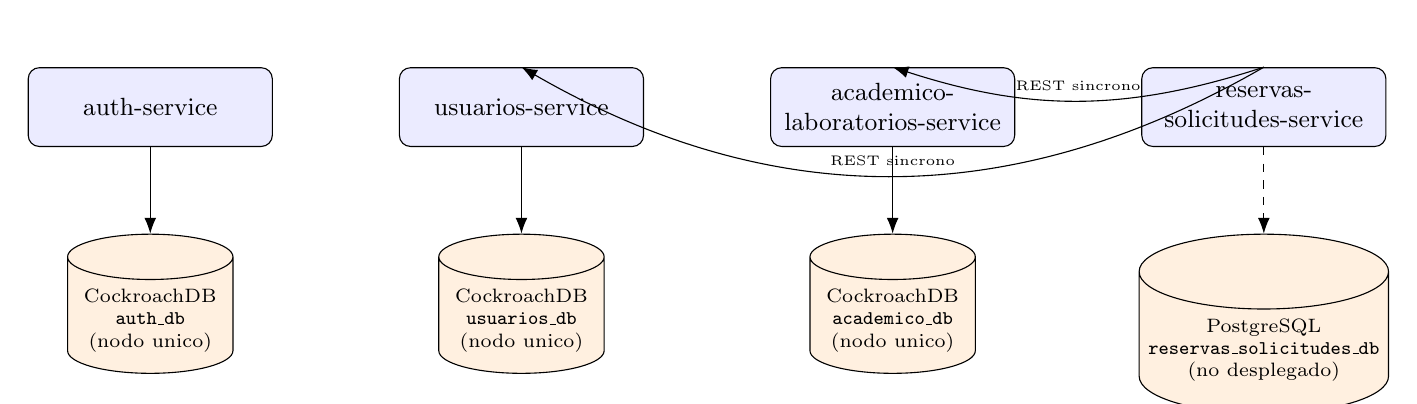
\begin{tikzpicture}[
    node distance=1.1cm and 1.6cm,
    svc/.style={rectangle, rounded corners, draw, fill=blue!8, minimum width=3.1cm, minimum height=1cm, align=center, font=\small},
    db/.style={cylinder, shape border rotate=90, draw, fill=orange!12, minimum width=2.1cm, minimum height=1.1cm, align=center, font=\scriptsize, aspect=0.3},
    ext/.style={rectangle, rounded corners, draw, fill=gray!10, minimum width=3.1cm, minimum height=0.9cm, align=center, font=\small}
]
\node[svc] (auth) {auth-service};
\node[svc, right=of auth] (usu) {usuarios-service};
\node[svc, right=of usu] (aca) {academico-\\laboratorios-service};
\node[svc, right=of aca] (res) {reservas-\\solicitudes-service};

\node[db, below=of auth] (dbauth) {CockroachDB\\\texttt{auth\_db}\\(nodo unico)};
\node[db, below=of usu] (dbusu) {CockroachDB\\\texttt{usuarios\_db}\\(nodo unico)};
\node[db, below=of aca] (dbaca) {CockroachDB\\\texttt{academico\_db}\\(nodo unico)};
\node[db, below=of res] (dbres) {PostgreSQL\\\texttt{reservas\_\-solicitudes\_db}\\(no desplegado)};

\draw[-{Latex[length=2mm]}] (auth) -- (dbauth);
\draw[-{Latex[length=2mm]}] (usu) -- (dbusu);
\draw[-{Latex[length=2mm]}] (aca) -- (dbaca);
\draw[dashed, -{Latex[length=2mm]}] (res) -- (dbres);

\draw[-{Latex[length=2mm]}, bend left=18] (res.north) to node[above, font=\tiny, sloped] {REST sincrono} (aca.north);
\draw[-{Latex[length=2mm]}, bend left=30] (res.north) to node[above, font=\tiny, sloped] {REST sincrono} (usu.north);

\end{tikzpicture}
\caption{Topologia de datos de SCLI: patron de base de datos por servicio. Cada microservicio posee un limite transaccional propio y una instancia de base de datos exclusiva; \texttt{reservas-solicitudes-service} consulta a \texttt{academico-laboratorios-service} y a \texttt{usuarios-service} mediante llamadas REST sincronas sin transaccion distribuida. El cuarto servicio (linea discontinua) aun no forma parte del despliegue orquestado con \texttt{docker-compose}.}
\label{fig:topologia}
\end{figure}

\subsection{Consistencia dentro del limite de cada microservicio}

Dentro del limite transaccional de \texttt{reservas-solicitudes-service} -- el componente donde reside la logica de negocio mas sensible a condiciones de carrera -- el modelo implementado corresponde a consistencia fuerte de tipo serializable, reforzada por dos mecanismos complementarios observables directamente en el codigo.

Primero, control de concurrencia optimista mediante versionado: las entidades \texttt{SolicitudReserva}, \texttt{Reserva}, \texttt{BloqueoAgenda} y \texttt{ConfiguracionReserva} incorporan un campo \texttt{version} anotado con \texttt{@Version} de JPA/Hibernate. Segun el documento de diseño de la maquina de estados del propio equipo, la cancelacion concurrente de una reserva \emph{"se controla con el campo version mediante versionado optimista"}, de modo que si dos solicitudes de cancelacion compiten por la misma reserva, la que pierde la carrera no puede sobrescribir el estado vigente y recibe una respuesta de conflicto. Este mecanismo evita, sin necesidad de bloqueos pesimistas permanentes, que dos actores modifiquen concurrentemente el mismo agregado sin darse cuenta uno del otro.

Segundo, atomicidad de agregado mediante transaccion local unica: la aprobacion de una solicitud -- que cambia su estado a \texttt{APROBADA}, crea exactamente una \texttt{Reserva} en estado \texttt{PROGRAMADA} y registra el evento en \texttt{HistorialSolicitud} -- esta explicitamente definida como una unica operacion de negocio que debe ejecutarse en la misma transaccion local, revirtiendose por completo si cualquiera de sus efectos falla. La misma exigencia se aplica a la cancelacion de una solicitud aprobada, que debe cambiar de estado tanto la solicitud como su reserva asociada dentro de una unica transaccion. Este diseño evita, por construccion, estados intermedios inconsistentes como una solicitud aprobada sin reserva asociada o una reserva huerfana sin solicitud.

A esto se suma el uso de una cabecera \texttt{Idempotency-Key}, obligatoria en las operaciones de creacion y aprobacion de solicitudes, que protege al sistema frente a reintentos de red: una misma clave de idempotencia repetida no debe producir efectos duplicados, propiedad indispensable en un sistema distribuido donde el cliente no siempre puede saber con certeza si una peticion previa tuvo exito en el servidor.

En conjunto, dentro de cada microservicio SCLI implementa un modelo cercano a la linealizabilidad para las operaciones que modifican el agregado \texttt{SolicitudReserva}/\texttt{Reserva}: cualquier lector posterior a una escritura confirmada observa el efecto de esa escritura, porque no existe replica secundaria dentro del mismo servicio que pueda quedarse atras (el despliegue es de nodo unico) y porque el aislamiento serializable de CockroachDB, combinado con el versionado optimista de la aplicacion, impide anomalias de escritura concurrente.

\subsection{Consistencia entre microservicios}

El panorama cambia en la frontera entre servicios. Cuando \texttt{reservas-solicitudes-service} necesita verificar la existencia de un laboratorio o la disponibilidad de un docente, invoca sincronamente a \texttt{academico-laboratorios-service} y a \texttt{usuarios-service} mediante clientes REST configurados con tiempos de espera y reintentos (\texttt{RestClientConfig}, \texttt{AcademicoLaboratoriosClient}, \texttt{UsuariosClient}). No existe entre estos servicios ninguna transaccion distribuida, protocolo de confirmacion en dos fases ni mensajeria asincrona: el repositorio no contiene dependencias de Kafka, RabbitMQ ni ningun otro middleware de mensajeria. Los propios documentos de diseño del equipo son explicitos al respecto: las referencias externas como \texttt{laboratorioId} o \texttt{solicitanteId} se almacenan como valores UUID \emph{"sin claves foraneas hacia bases de datos externas y sin relaciones ORM locales"}, y su validez \emph{"se resolvera mediante los contratos de integracion correspondientes, no mediante integridad referencial entre bases"}.

Esta decision de diseño equivale, en terminos del espectro de la Seccion 4.1, a un modelo de consistencia debil entre servicios -- mas cercano a la consistencia eventual acotada por contrato que a cualquier garantia fuerte -- con una ventana de posible obsolescencia entre el instante en que \texttt{reservas-solicitudes-service} consulta el estado de un laboratorio (\texttt{DisponibilidadController}) y el instante en que aprueba una solicitud sobre ese mismo laboratorio. Si \texttt{academico-laboratorios-service} cambia el estado de un laboratorio a inactivo entre ambas llamadas, no existe ningun mecanismo de coordinacion distribuida que lo impida a nivel de infraestructura; la coherencia depende de que la aplicacion vuelva a validar la condicion en el momento de aprobar, no de una garantia transaccional entre bases de datos. Es, en esencia, el mismo compromiso que describe la formulacion PACELC para el eje Else-Latencia-Consistencia: el equipo opto por baja latencia y desacoplamiento entre servicios en operacion normal, aceptando una consistencia mas debil en las lecturas entre limites de servicio.

% ==========================================================
% 4. EVALUACION DE ALTERNATIVAS
% ==========================================================
\section{Evaluacion de alternativas y trade-offs}

Para responder si el modelo vigente es el optimo, se contrastan a continuacion dos alternativas concretas frente al modelo actualmente implementado.

\textbf{Alternativa 1 -- Sagas coreografiadas con mensajeria asincrona.} En lugar de que \texttt{reservas-solicitudes-service} invoque sincronamente a los demas servicios y valide en el mismo hilo de peticion, el flujo de aprobacion se modelaria como una saga: cada paso (reservar horario, validar disponibilidad de laboratorio, notificar) se publica como evento en un broker (por ejemplo Kafka o RabbitMQ) y cada servicio reacciona de forma asincrona, con una accion de compensacion explicita si un paso posterior falla (por ejemplo, liberar la reserva si la validacion academica llega negativa). Este patron es el que sistemas orientados a disponibilidad, como Dynamo, generalizan mediante resolucion de conflictos y reconciliacion posterior en lugar de coordinacion previa \cite{decandia2007}.

\textbf{Alternativa 2 -- Clúster CockroachDB realmente distribuido (multinodo).} Sin cambiar el modelo de programacion actual, se sustituirian las instancias \texttt{start-single-node} por un despliegue de al menos tres nodos por servicio, habilitando la replicacion Raft real entre ellos. El modelo de consistencia dentro de cada servicio no cambiaria -- seguiria siendo serializable -- pero pasaria de ser una propiedad teorica del motor a una garantia efectiva con tolerancia a fallos de nodo, acercando el comportamiento del sistema al de Spanner, del cual CockroachDB desciende conceptualmente \cite{corbett2013}.

La Tabla~\ref{tab:comparacion} contrasta ambas alternativas con el modelo actual segun cinco criterios tecnicos.

\begin{table}[htbp]
\centering
\small
\caption{Comparacion del modelo actual de SCLI frente a dos alternativas de consistencia y replicacion.}
\label{tab:comparacion}
\begin{tabular}{@{}p{2.6cm}p{3.1cm}p{3.6cm}p{3.6cm}@{}}
\toprule
\textbf{Criterio} & \textbf{Modelo actual} & \textbf{Alt. 1: Sagas asincronas} & \textbf{Alt. 2: Cockroach multinodo} \\
\midrule
Consistencia & Fuerte intra-servicio (serializable); debil entre servicios (sin compensacion) & Eventual explicita entre servicios, con compensacion definida & Fuerte intra-servicio, igual que hoy; no mejora la frontera entre servicios \\
\addlinespace
Disponibilidad & Media: una llamada REST caida bloquea la operacion completa & Alta: los servicios se desacoplan temporalmente entre si & Alta dentro de cada servicio: tolera caida de un nodo sin perder el servicio \\
\addlinespace
Latencia & Baja-media: suma de latencias de llamadas sincronas encadenadas & Baja percibida por el cliente, pero mayor tiempo hasta consistencia final & Baja-media, ligeramente mayor que nodo unico por el consenso Raft real \\
\addlinespace
Tolerancia a particiones & Baja: una particion hacia \texttt{academico-laboratorios-service} detiene la aprobacion & Alta: los eventos se reintentan cuando la particion se resuelve & Alta: el clúster sigue disponible si falla una minoria de nodos \\
\addlinespace
Complejidad & Baja: llamadas REST directas, facil de razonar y depurar & Alta: exige broker, logica de compensacion y observabilidad distribuida & Media: solo cambia infraestructura de despliegue, no logica de aplicacion \\
\bottomrule
\end{tabular}
\end{table}

Las dos alternativas no son mutuamente excluyentes ni compiten por el mismo problema: la Alternativa 2 resuelve la fragilidad de la replicacion \emph{dentro} de cada servicio, mientras que la Alternativa 1 resuelve la fragilidad de la coordinacion \emph{entre} servicios. Esta distincion es la base de la discusion critica de la Seccion 6.

% ==========================================================
% 5. DISCUSION CRITICA
% ==========================================================
\section{Discusion critica: ¿es el modelo optimo?}

La respuesta a la pregunta orientadora no es uniforme para todo el sistema, porque SCLI en realidad contiene dos modelos de consistencia distintos segun el nivel al que se observe.

Dentro del agregado \texttt{SolicitudReserva}/\texttt{Reserva}, el modelo elegido -- consistencia serializable respaldada por versionado optimista y transacciones locales atomicas -- es tecnicamente adecuado para el dominio. El costo de una anomalia de consistencia en este punto (dos reservas aprobadas para el mismo laboratorio y horario) es alto y dificil de revertir socialmente una vez que los usuarios han sido notificados, mientras que el costo de rechazar ocasionalmente una operacion concurrente con un \texttt{409 Conflict} es bajo: el usuario simplemente reintenta. Leido bajo PACELC, el equipo eligio consistencia sobre latencia en el eje Else, lo cual es coherente con un dominio donde las operaciones de escritura sobre una misma reserva son poco frecuentes por recurso individual y donde la correctitud importa mas que los milisegundos de respuesta.

Sin embargo, dos limitaciones concretas impiden calificar el modelo completo como optimo en su estado actual. La primera es el despliegue en nodo unico: el motor CockroachDB fue elegido precisamente por su capacidad de ofrecer consistencia fuerte con replicacion distribuida, pero esa capacidad no esta siendo utilizada. Bajo el eje P de CAP, una particion o caida del unico nodo de \texttt{academico\_db} no se traduce en un compromiso entre consistencia y disponibilidad, sino en indisponibilidad total del servicio, que es precisamente el resultado que la replicacion deberia evitar. La mitigacion es directa y de bajo costo relativo: la Alternativa 2 no exige reescribir logica de aplicacion, solo cambiar la configuracion de despliegue.

La segunda limitacion es estructural: la ausencia de compensaciones formales entre \texttt{reservas-solicitudes-service} y los servicios de los que depende. El propio diseño documental del equipo reconoce que la validez de las referencias externas se resuelve por contrato, no por integridad referencial, lo cual es una decision razonable en microservicios pero que traslada la responsabilidad de la consistencia a la logica de aplicacion en tiempo de peticion. Mientras el sistema sea de tamaño reducido y los servicios respondan con alta disponibilidad, esta ventana de obsolescencia entre validacion y aprobacion es improbable que se manifieste; a medida que el sistema escale o se agregue mayor concurrencia entre periodos de matricula, esa ventana deja de ser un riesgo teorico. La mitigacion recomendada no es necesariamente adoptar la Alternativa 1 de inmediato -- su complejidad operativa es alta para el tamaño actual del equipo -- sino, como paso intermedio, revalidar explicitamente el estado del laboratorio dentro de la misma transaccion de aprobacion y documentar el comportamiento esperado ante una respuesta tardia o fallida del servicio academico, antes de considerar mensajeria asincrona como evolucion futura.

En sintesis, el modelo de consistencia de SCLI es parcialmente optimo: acertado en la decision central de proteger el agregado de reserva con consistencia fuerte, e insuficiente en dos aspectos de implementacion -- replicacion fisica no explotada y coordinacion entre servicios no formalizada -- que son subsanables sin cambiar la arquitectura de fondo. Ninguna de las dos limitaciones invalida la eleccion del modelo; ambas senalan una brecha entre el modelo de consistencia que el diseño del equipo declara perseguir y el que el despliegue actual efectivamente garantiza.

% ==========================================================
% 6. CONCLUSIONES
% ==========================================================
\section{Conclusiones}

\begin{enumerate}[label=\arabic*.]
\item SCLI implementa el patron de base de datos por servicio sobre un motor -- CockroachDB -- diseñado para ofrecer consistencia fuerte mediante replicacion basada en consenso, en la linea de Spanner, aunque su despliegue actual como nodo unico no explota todavia esa capacidad.

\item Dentro del limite transaccional de cada microservicio, en particular en \texttt{reservas-solicitudes-service}, el modelo implementado combina aislamiento serializable, control de concurrencia optimista por version y transacciones locales atomicas, lo que produce garantias cercanas a la linealizabilidad para el agregado solicitud-reserva, adecuadas a un dominio donde la doble reserva de un mismo laboratorio es inaceptable.

\item Entre microservicios, la ausencia de transacciones distribuidas y de mensajeria asincrona con compensacion formal produce un modelo de consistencia debil, de tipo eventual acotado por contrato, con una ventana de obsolescencia entre la consulta de disponibilidad y la aprobacion de una solicitud.

\item Leido bajo CAP y PACELC, el sistema prioriza consistencia sobre latencia dentro de cada servicio y prioriza desacoplamiento y baja latencia sobre consistencia estricta entre servicios; ambas decisiones son defendibles para el dominio, pero la primera no esta completamente respaldada aun por la infraestructura de despliegue.

\item El modelo de consistencia elegido es parcialmente optimo para el dominio de SCLI: la eleccion conceptual es correcta, pero su realizacion esta incompleta mientras el proyecto continua en desarrollo, y las dos mitigaciones identificadas -- despliegue multinodo y revalidacion transaccional entre servicios -- son de complejidad manejable para el estado actual del equipo.
\end{enumerate}

% ==========================================================
% 7. DECLARACION DE USO DE IA GENERATIVA
% ==========================================================
\section{Declaracion de uso de IA generativa}

Para la elaboracion de este informe se utilizo puntualmente la herramienta Claude (Anthropic), unicamente como apoyo en dos tareas especificas: (i) revision del codigo fuente y la configuracion de despliegue del repositorio del PFC SCLI (\repoPFC) -- en particular el archivo \texttt{docker-compose.yml}, las entidades y controladores de \texttt{reservas-solicitudes-service} y los documentos de diseño de dominio del equipo -- para verificar con precision tecnica el motor de base de datos, la estrategia de replicacion y los mecanismos de concurrencia efectivamente implementados antes de caracterizarlos en la Seccion 5; y (ii) contraste de las alternativas de la Seccion 6 frente al modelo actual, para asegurar que los criterios de comparacion fueran tecnicamente consistentes con la literatura citada. La redaccion, el analisis critico, la postura frente a la pregunta orientadora y las conclusiones del informe son elaboracion propia del estudiante, quien conoce el PFC por participar en su desarrollo y valido cada afirmacion tecnica contra el repositorio fuente antes de la entrega.

\newpage
% ==========================================================
% REFERENCIAS (IEEE)
% ==========================================================
\begin{thebibliography}{9}

\bibitem{abadi2012}
D. J. Abadi, ``Consistency Tradeoffs in Modern Distributed Database System Design: CAP is Only Part of the Story,'' \emph{Computer}, vol. 45, no. 2, pp. 37--42, 2012. doi: 10.1109/MC.2012.33

\bibitem{corbett2013}
J. C. Corbett \emph{et al.}, ``Spanner: Google's Globally Distributed Database,'' \emph{ACM Transactions on Computer Systems}, vol. 31, no. 3, pp. 1--22, 2013, art. no. 8. doi: 10.1145/2491245

\bibitem{decandia2007}
G. DeCandia \emph{et al.}, ``Dynamo: Amazon's Highly Available Key-value Store,'' in \emph{Proc. 21st ACM SIGOPS Symposium on Operating Systems Principles (SOSP '07)}, 2007, pp. 205--220. doi: 10.1145/1294261.1294281

\bibitem{gilbert2002}
S. Gilbert and N. Lynch, ``Brewer's Conjecture and the Feasibility of Consistent, Available, Partition-Tolerant Web Services,'' \emph{ACM SIGACT News}, vol. 33, no. 2, pp. 51--59, 2002. doi: 10.1145/564585.564601

\bibitem{vansteen2017}
M. van Steen and A. S. Tanenbaum, \emph{Distributed Systems}, 3rd ed. distributed-systems.net, 2017, isbn: 978-1543057386.

\bibitem{viotti2016}
P. Viotti and M. Vukolic, ``Consistency in Non-Transactional Distributed Storage Systems,'' \emph{ACM Computing Surveys}, vol. 49, no. 1, pp. 1--34, 2016, art. no. 19. doi: 10.1145/2926965

\end{thebibliography}

\end{document}
